\documentclass{article}
\author{Allen W. Lynch}
\title{Locus Regression}
\date{\today}
\newcommand{\Lagr}{\mathcal{L}}
\newcommand{\dgfunc}{\mathcal{\psi}}
\usepackage{amsfonts}
\usepackage{algorithm,algorithmic}
\usepackage{amsmath}
\usepackage{graphicx}
\graphicspath{ {./figures/} }
\newcommand{\surrB}{\hat{\Lagr}^{(\beta)}_{\zeta}}


\begin{document}
\maketitle

\section{Introduction}

\section{Generative Model}

The generative model explains the observed mutations in a dataset of $G$ genomes, where mutations in a genome are composed of a 
distribution over $K$ signatures, or processes, each of which has a characteristic bias with respect to which genomic loci and nucleotides it affects. 
Mutations in genome $g$ are expressed as tuples of $(m,\ell)$, where $m \in \{ m \in \mathbb{Z} | 1 \leq m \leq 96\}$ is the trinucleotide context and the mutation (of which there are 96 possibilities)
and $\ell \in \{ \ell \in \mathbb{Z} | 1 \leq \ell \leq L \}$ is the genomic locus or window at which that mutation occurred, with $L$ possible windows. 
In the generative process outlined below, $\pi_g \in \mathbb{R}_{(0,1)}^K, \sum_{k=1}^K \pi_{gk} = 1$ is the composition over processes that generated the mutations in a genome $g$,
$N_g$ is the number of mutations in $g$, and $z$ is an indicator variable which describes which process generated the $i^{th}$ mutation:

\begin{algorithm}
\caption{Generative Process}
\begin{algorithmic}
  \scriptsize
  \FORALL{$g \in {1...G}$}
  	\STATE $ \pi_g \sim \textrm{Dirichlet}( \alpha ) $
  	\FORALL{$i \in {1...N_g}$}
  		\STATE $ z_{gi} \sim \textrm{Categorical}( \pi_g ) $
  		\STATE $ \ell_{gi} \sim \textrm{Categorical}( \theta_{z_{gi},g} ) $
  		\STATE $ m_{gi} \sim \textrm{Categorical}( \psi_{z_{gi},\ell_{gi}} ) $
  	\ENDFOR
  \ENDFOR
\end{algorithmic}
\end{algorithm}

Like the closely-related process for generating a textual corpus utilized by Latent Dirichlet Allocation (LDA), we sample the mutations in a genome by
iteratively choosing a process ($z$), then a locus ($\ell$) and a mutation ($m$) from categorical distributions. Unlike LDA, however, the distribution over loci $\theta$ 
is conditioned on both process \emph{and} sample effects - for a given process, the distribution over loci may be different across samples. For example, a process which
affects nucleotides in heterochromatin will have a different distribution over loci for two samples with different epigenetic states. Learning a distribution over loci for 
each process in each sample by estimating $\theta$ for each $z,g$ would have extremely high variance.
Therefore, we estimate $\theta$ using a data efficient parameterization which describes how a process acts across loci and samples with respect to genomic correlates (see section \textbf{3}).

Likewise, the distribution over mutations, $\psi$, is conditioned on the process \emph{and} the locus, since different genomic windows may have different 
distributions over trinucleotide contexts on which a process acts. Again, we must construct a data-efficient parameterization for this distribution (see section \textbf{4}).


\section{Parameterizing $\theta$}

As outlined above, the distribution of mutations over loci for each process and sample is high-dimensional and impractical to compute directly. Instead, we paramterize this
distribution in terms of a simpler model of process-dependent mutation rates. We assume that the probability of a mutation occurring at a locus given a process $z$ and a sample $g$ is proportional to the estimated mutation rate for that locus. We predict mutation rate using a linear model where loci are associated with genomic features $X^{(g)} \in \mathbb{R}^{F,L}$, where $L$ is the number of loci and $F$ is the number of features, and processes have coefficients $\beta_z \in \mathbb{R}^{F}$. Thus, 

\begin{equation} \label{3}
p(\ell | z, g) = (\theta_{z,g})_\ell \propto l_\ell  \textrm{exp}(\sum_{f=1}^{F}\beta_{zf} X^{(g)}_{f\ell}) = l_\ell \textrm{exp}(\beta_z^T X^{(g)}_\ell)
\end{equation}

Above, $l_\ell$ is the length in nucleotides for that window, but this parameter can also represent user-specified "exposure" variables. For instance, $\ell$ may adjust for technical effects which influence the sensitivity to call mutations within a window independent of the mutation rate.

Notably, the features $X$ are dependent on the sample $g$, while $\beta$ only depends on the process. In this way, this parameterization can capture jointly process and sample-specific variation in mutation rate across the genome using few parameters. To specify a valid probability distribution over $\ell$, we must introduce some multiplicative normalizer to the mutation rate model. That normalizer is the sum of predicted mutation rates across all loci:

\begin{equation}
p(\ell | z, g) = \frac{1}{\sum_{\ell'=1}^L l_{\ell'} \textrm{exp}(\beta_z^T X^{(g)}_{\ell'})} l_\ell \textrm{exp}(\beta_z^T X^{(g)}_\ell)
\end{equation}


Finally, to regularize the coefficients and address uncertainty in the posterior estimate of $\theta$, we treat $\beta$ as a random variable with prior:

\begin{equation}
\beta_{zf} \sim \textrm{Normal}(0,\tau^2_z)
\end{equation}


\section{Parameterizing $\psi$}

The distribution $\psi$ gives the probability of each mutation - defined by the trinucleotide context and alternative nucleotide - occuring given some process $z$ and genomic window $\ell$. We assume that the dependence on $\ell$ is solely the result of differences in available contexts to mutate within windows, and that the $\theta$ distribution fully explains all other locus-based effects.

We factorize the process of generating a single mutation into two components: a distributions over contexts, $c$, from the set $\mathbb{C}$ of trinucleotide contexts (of which there are 32) and a distribution over alternative nucleotides, $a$, conditioned on that context. The set of alternative nucleotides $\mathbb{A}_c$ is defined as $\{ a \in \{\mathrm{A, T, C, G}\} | a \neq c_{\mathrm{ref}}\}$ which excludes the middle nucleotide of the context ($c_{\mathrm{ref}}$), since a nucleotide cannot mutate to itself. As an example, the probability of a mutation expressed in the COSMIC notation is given by:

\begin{equation}
P(m = \textrm{A[C:T]G} | z, \ell) = P(a=\textrm{T} | z, c=\textrm{ACG}) P(c=\textrm{ACG} | z, \ell)
\end{equation}

We assume that each mutational process acts on each nucleotide context at some fixed rate, $\lambda_{zc} \in \mathbb{R}_{(0,\inf)}$, such that over some arbitrary timestep and acting in a locus $\ell$ with $ t_{\ell c}$ such contexts, $\lambda_{zc}\cdot t_{\ell c}$ of them are mutated.

Assuming the reserve of contexts cannot be depleted, the portion of mutated contexts of some type is given by:

\begin{equation}
p(c | z, \ell) = \frac{\lambda_{zc}t_{\ell c}}{\sum_{c'\in \mathbb{C}} \lambda_{zc'}t^{T}_{c' \ell}} 
\end{equation}

Given a context and a process, the distribution over alternative nucleotides is:

\begin{equation}
p(a | z, c) = \rho_{zca}, \sum_{a \in \mathbb{A}_c} \rho_{zca} = 1
\end{equation}

We treat $\lambda \in \mathbb{R}^{K \times |\mathbb{C}|}_{(0,1)}$ as a collection of Gamma-distributed random variables. Above, we cast the problem as inferring absolute rates, which is impossible from the data. If instead, we infer relative rates:

\begin{equation}
p(c | z, \ell) = 
\left( \frac{\frac{1}{\sum_{c'=1}^{C} \lambda_{zc'}}}{\frac{1}{\sum_{c'=1}^{C} \lambda_{zc'}}} \right) \cdot \frac{\lambda_{zc}t_{\ell c}}{\sum_{c'=1}^{C} \lambda_{zc'}t^{T}_{c' \ell}} 
\end{equation}

Then the random variable $\frac{\lambda_{zc}}{\sum_{c'=1}^{C} \lambda_{zc'}} \forall c \in \{1 ... |\mathbb{C}|\}$ is Dirichlet-distributed under the condition the underlying Gamma distributions share the same rate variable. 

\section{Variational inference}

For a corpus of genomes with mutations, each genome has a composition over mutational processes $\pi_g\forall g \in \{1...G\}$ drawn from a Dirichlet prior: $\pi_g \sim \mathrm{Dir}(\alpha)$. Each genome has mutations $m_{gi}$ at loci $\ell_{gi}$ associated with a hidden process variable $z_{gi} \forall i \in \{1...N_g\}$. Finally, the random variables associated with the nucleotide signature of each mutational process, $\rho$ and $\lambda$, are drawn from uniform Dirichlet priors, and the random variable $\beta$ is drawn from prior parameterized by the parameter $\tau$. Altogether, the joint PDF of the model is:

\begin{align*}
p_{\alpha,\tau}(m,l,z,\beta,\pi,\lambda,\rho) = p(\lambda | \textbf{1})p(\rho | \textbf{1})p(\beta | \tau) \\
	 \prod_{g=1}^G p( \pi_g | \alpha ) \prod_{i=1}^{N_g} p(m_{gi} | \ell_{gi}, \lambda_{z_{gi}}, \rho_{z_{gi}} ) p( \ell_{gi} | \beta_{z_{gi}} ) p(z_{gi} | \pi_g )
\end{align*}

Direct inference of the posterior distribution over model parameters is intractable, so we employ variational inference to infer an approximate posterior. Particularly,
we assume the parameter posterior densities are independent and are specified by variational parameters such that:

\begin{align}
p(\pi,\lambda,\rho,\beta,z | m, l) \approx \prod_{k=1}^K q(\lambda_k; \delta_k)q(\rho_k; \omega_k)q(\beta_k; \mu_k, \nu_k) \\
	\prod_{g=1}^G q(\pi_g; \gamma_g) \prod_{i=1}^{N_g} q(z_{gi};\phi_{gi})
\end{align}

\begin{align*}
\lambda_k \sim q(.;\delta_k) = \textrm{Dir}(\delta_k) \\
	\rho_k \sim q(.;\omega_k) = \textrm{Dir}(\omega_k) \\
	\beta_k \sim q(.;\mu_k, \nu_k) = \textrm{Normal}(\mu_k, \nu_k^2) \\
	\pi_g \sim q(.;\gamma_g) = \textrm{Dir}(\gamma_g) \\
	z_{gi} \sim \textrm{Categorical}(\phi_{gi})
\end{align*}

To infer the optimal values of the variational parameters, $\Omega^* = \{\delta^*, \omega^*, \mu^*, \nu^*, \gamma^*, \phi^*\}$, we optimize with respect to:

\begin{equation}
\Omega^* = \mathrm{argmin}_{\Omega} D_{KL}( q(.;\Omega) || p(.| m, \ell) )
\end{equation}

Or equivalently:

\begin{equation} \label{1}
\Omega^* = \mathrm{argmax}_{\Omega} E_{q(.;\Omega)}[\log p_{\alpha,\tau}(m,l, \pi, \lambda, \beta, z)] + \mathcal{H}(q(.;\Omega))
\end{equation}

Expanding the terms in \eqref{1}, we define the objective function:

\begin{equation} \label{L}
\begin{split}
\Lagr(\delta, \omega, \mu, \nu, \gamma, \phi) = \\
	E_q [\log p(\beta | \tau)] + E_q [\log{p(\pi | \alpha)}] +  E_q [\log{p(z | \pi )}] + \\
	E_q [\log{p(\ell | z, \beta)}] + E_q [\log{p(m | \ell, z, \lambda, \rho)}] \\
	+ \mathcal{H}(q(z;\phi)) + \mathcal{H}(q(\lambda;\delta)) + \mathcal{H}(q(\rho;\omega)) + \mathcal{H}(q(\beta;\mu, \nu)) + \mathcal{H}(q(\pi|\gamma)) 
\end{split}
\end{equation}

Above, we omit the terms $E_q[\log p(\rho| \textbf{1})]$ and $E_q[\log p(\lambda| \textbf{1})]$. Since the prior gives a uniform distribution over all values of $\rho$, $\lambda$ these are constant terms.

We optimize the variational parameters in $\Lagr$ using the "Expectation Maximization" (EM) algorithm: we iteratively fix global parameters $\delta, \omega, \mu, \nu$ and find optimal local parameters $\gamma, \phi$ (E-step), then fix $\phi$ and find optimal global parameters (M-step). This process is guaranteed to find a stable local optimum with respect to $\Lagr$.


\subsection{M-step: Optimization of $\mu$, $\nu$}

Here we describe the method to find the optimal distribution for $\beta$, parameterized by $\mu$,$\nu$, while holding the other parameters fixed.

First, we subset \eqref{L} to only terms which depend on $\mu$, $\nu$, plug in \eqref{3}, and propagate the expectation by linearity. Below, the notation $X^{(g)}_{[\ell]_{gi}}$ refers to the operation of selecting the row of $X^{(g)}$ which corresponds with the observed locus of the $gi^\mathrm{th}$ mutation:

\begin{equation}
\begin{split}
\Lagr^{(\beta)} = E_q[p(\beta | \tau^2)] + E_q[\log p(\ell | \beta, z)] + \mathcal{H}(q(\beta;\mu, \nu)) \\
	= -\frac{1}{2\tau^2}\sum_{k=1}^K \sum_{f=1}^F \left( \mu_{kf}^2 + \nu_{kf}^2 \right) \\
	+ \sum_{g=1}^G \sum_{i=1}^{N_g} \sum_{k=1}^K  \phi_{gik} \left[ E_{\beta_k \sim q(.;\mu_k,\nu_k)} [\beta_k^T X^{(g)}_{[\ell]_{gi}}] - E_{\beta_k \sim q(.;\mu_k,\nu_k)} [\log{\sum_{\ell'=1}^L l_{\ell'} \textrm{exp}( \beta_k^T X^{(g)}_{\ell'} )}] \right] \\
	+ \sum_{k=1}^K \sum_{f=1}^F \log \nu_{kf}
\end{split}
\end{equation}

Via Jensen's inequality, we lower bound the objective function:

\begin{equation}
\begin{split}
\Lagr^{(\beta)} \geq \sum_{k=1}^K \sum_{f=1}^F -\frac{1}{2\tau^2}\left(\mu_{kf}^2 + \nu_{kf}^2 \right) + \log \nu_{kf} + \\
	\sum_{g=1}^G \sum_{i=1}^{N_g} \sum_{k=1}^K  \phi_{gik} \left[ \mu_k^T X^{(g)}_{[\ell]_{gi}} - \log{\sum_{\ell'=1}^L l_{\ell'} \textrm{exp}\{ \mu_k^T X^{(g)}_{\ell'} + \frac{1}{2}(\nu_k^T X^{(i)}_{\ell'})^2\}} \right]
\end{split}
\end{equation}

We cannot find optimal values for $\mu$,$\nu$ analytically, so we use gradient descent. Again, we define a lower-bound on the objective with the introduction of the $\zeta \in \mathbb{R}^K$ parameter. This removes the $\sum\exp$ term from the $\log$ and greatly simplifies calculation of the derivative. Below, we consider the scenario where every sample has the same genomic correlates (all samples have homogenous gene expression, chromatin accessibility, etc.), which simplifies the calculations. 

\begin{equation} \label{obj}
\begin{split}
\Lagr^{(\beta)} \geq \hat{\Lagr}^{(\beta)}_{\zeta}(\mu,\nu) = \sum_{k=1}^{K}\sum_{f=1}^F  -\frac{1}{2\tau^2}(\mu_{kf}^2 + \nu_{kf}^2) + \log{\nu_{kf}} \\
	+ \sum_{\ell=1}^L \left(\sum_{g=1}^G\sum_{i=1}^{N_g} \phi_{gik} \mathbb{I}_{[\ell]_{gi} = \ell} \right) \mu_k^T X_{\ell} \\
	- \frac{ \sum_{g=1}^G\sum_{i=1}^{N_g} \phi_{gik} }{\zeta_k}  \sum_{\ell'=1}^L l_{\ell'}\textrm{exp}\{ \mu_k^T X_{\ell'} + \frac{1}{2}(\nu_k^T X_{\ell'})^2\} + 1 - \log{\zeta_k}
\end{split}
\end{equation}

The first line of \eqref{obj} serves to regularize the values of $\mu$ and $\nu$. Intuitively, the regularizer of $\nu$ is a concave function defined over the positive reals with a maximum at $\nu = \tau$. 

\begin{figure}[h]
\caption{Function $-\frac{1}{2\tau^2}\nu^2 + \log\nu$ for decreasing values of $\tau$}
\centering
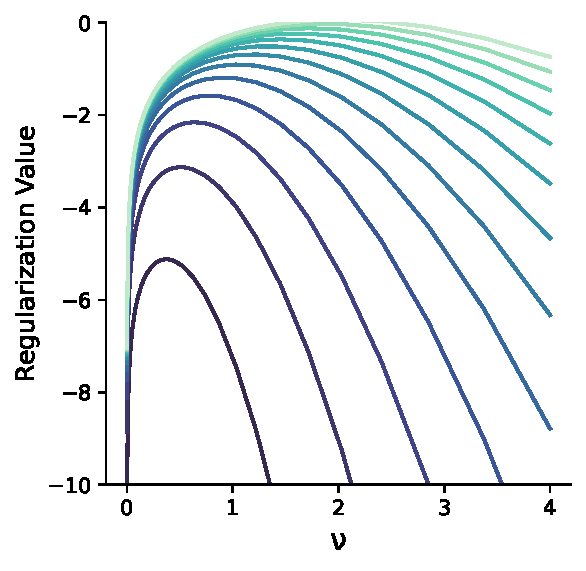
\includegraphics[scale=0.65]{nu_regularization.pdf}
\end{figure}

The second line of \eqref{obj} shows the sufficient statistics to update the variational parameters of $\beta$ are the number of mutations that fall within each locus weighted by the probability that mutation was generated by process $k$. To optimize, we first update $\zeta$:

\begin{equation}
\zeta_k = \sum_{\ell'=1}^L l_{\ell'}\textrm{exp} \left\{ \mu_k^T X_{\ell'} + \frac{1}{2}(\nu_k^T X_{\ell'})^2 \right\}
\end{equation}

then provide $\surrB$ and analytical derivatives $\frac{\partial\surrB}{\partial\mu}$, and $\frac{\partial\surrB}{\partial\nu}$ to \emph{scipy}'s L-BFGS-B optimization function.


\subsection{M-step: optimization of $\delta$, $\omega$ }

$ E_q [\log{p(m | \ell, z, \lambda, \rho})] = E_{\rho \sim q(.;\omega)} [\log p(a|z,c,\omega)] + E_{\lambda \sim q(.;\delta)} [\log p(c|z,\ell,\lambda) ]$

$\Lagr^{(\delta)} = E_{\lambda \sim q(.;\delta)} [\log p(c|z,\ell,\lambda)] + \mathcal{H}(q(\lambda; \delta)) $

\begin{equation}
\begin{split}
\Lagr^{(\delta)} \geq \sum_{k=1}^K \sum_{c=1}^{|\mathbb{C}|} \left(\sum_{g=1}^G\sum_{i=1}^{N_g} \phi_{gik} \mathbb{I}_{[c]_gi = c}\right) \left( \Psi(\delta_{kc}) - 		\Psi(\sum_{c'=1}^{|\mathbb{C}|} \delta_{kc'}) \right) 
	\\ - \sum_{\ell=1}^L \left(\sum_{g=1}^G\sum_{i=1}^{N_g} \phi_{gik} \mathbb{I}_{[\ell]_{gi} = \ell} \right) \log{\sum_{c'=1}^{|\mathbb{C}|} \lambda_{kc'}(\sum \lambda_k)^{-1} t_{c'\ell}} \\
	+ \mathcal{H}(q(.;\delta))
\end{split}
\end{equation}


\begin{equation}
\mathrm{argmax}_{\omega_{ca}} E_{\rho \sim q(.;\omega)} [\log p(a|z,c,\omega)] + \mathcal{H}(q(\rho; \omega)) = \sum_{g=1}^G\sum_{i=1}^{N_g}\sum_{k=1}^K \phi_{gik} \mathbb{I}_{[c]_{gi} =c, [a]_{gi} = a} + 1
\end{equation}


\subsection{E-step: Optimization of $\gamma$, $\phi$}



\subsection{Stochastic Variational Inference}


\begin{figure}[h]
\caption{Bound convergence on training samples for PCAWG Esophogeal Adenocarcinoma Chr1 mutations dataset, colored by locus sampling rate (1 is no downsampling.)}
\centering
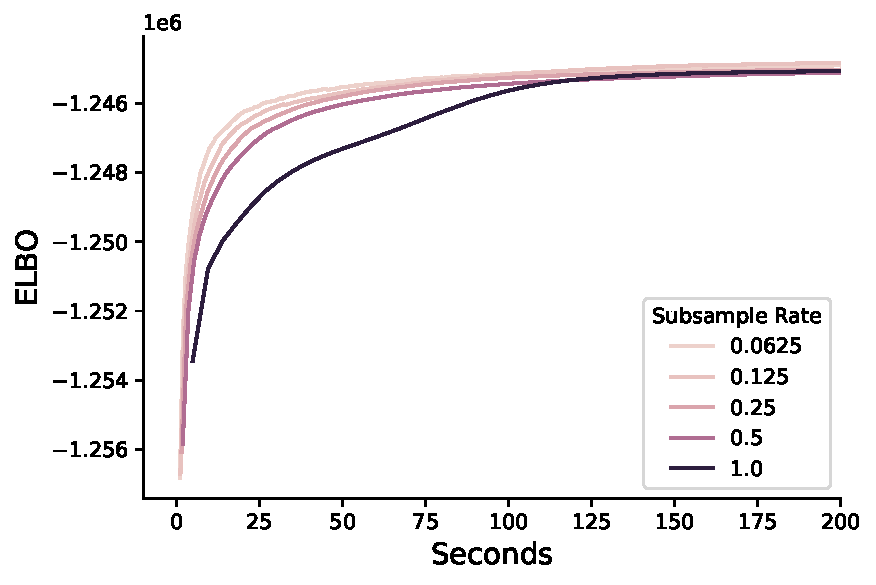
\includegraphics[scale=0.65]{svi_subsampling.pdf}
\end{figure}



\end{document}